\documentclass[tikz]{standalone}

\usepackage{xcolor}
\definecolor{hse-dunkelblau}{cmyk}{1,.7,.08,.54}  % HS Esslingen Dunkelblau (100 / 70 / 8 / 54)
\definecolor{hse-rot}{cmyk}{.1,1,.7,0}            % HS Esslingen Rot (10 / 100 / 70 / 0)
\definecolor{hse-hellblau}{cmyk}{.75,.1,.06,0}    % HS Esslingen Hellblau (75 / 10 / 6 / 0)
\definecolor{hse-blau75}{HTML}{8abde2}            % HS Esslingen Blau 75%
\definecolor{hse-blau50}{HTML}{b4d3ed}            % HS Esslingen Blau 50%
\definecolor{hse-blau25}{HTML}{dbe9f7}            % HS Esslingen Blau 25%
\definecolor{hse-blau15}{HTML}{eaf2fa}            % HS Esslingen Blau 15%
\definecolor{hse-hellgrau}{cmyk}{0,0,0,.08}       % HS Esslingen Hellgrau (0 /0 /0 /8)
\definecolor{dunkelgrau}{gray}{0.7}               % Dunkelgrau mit einem Grauwert von 70%
\definecolor{mittelgrau}{gray}{0.9}               % Mittelgrau mit einem Grauwert von 90%
\definecolor{hellgrau}{cmyk}{0,0,0,.08}           % Hellgrau (gleiche Werte wie hse-hellgrau)
\definecolor{dunkelblau}{cmyk}{1,.7,.08,.54}      % Dunkelblau (gleiche Werte wie hse-dunkelblau)
\definecolor{weiss}{cmyk}{0,0,0,0}                % Weiß

\begin{document}
  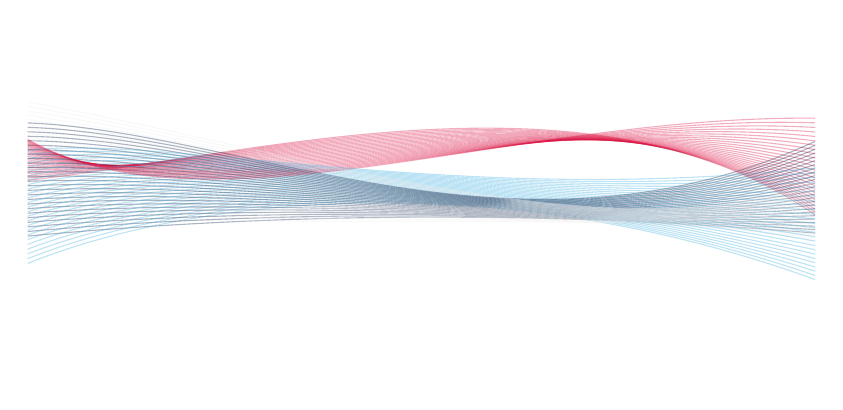
\begin{tikzpicture}[opacity=.35]
    \clip (1,-4) rectangle (11,0.5);
    \foreach \x in {0,0.06,...,1.5}{
      \draw[color=hse-rot] (0,\x-1.5) .. controls (3-0.6*\x,-1.5-\x) and (9-1.2*\x,0.8-0.7*\x) .. (12,-2.8+1.4*\x);
      \draw[color=hse-dunkelblau] (0,\x-2.25) .. controls (4-0.5*\x,\x-1.8) and (8-0.4*\x,-1.8-\x) .. (12,-2.2+1.2*\x);
      \draw[color=hse-hellblau] (0,\x-3) .. controls (2-0.7*\x,\x-1.7) and (7-0.8*\x,-0.9-0.8*\x) .. (12,-3.1+1.3*\x);
      \draw[color=hse-hellgrau] (0,\x-1.8) .. controls (5-0.9*\x,\x-2.2) and (10-0.3*\x,-1.6-\x) .. (12,-2.5+1.1*\x);
    }
  \end{tikzpicture}
\end{document}